\section{Implementation}
\label{sec:implementation}

We provide an implementation of our recurrent clustering algorithm in a tool called \textsc{ML4HS}, which consists of a loose collection of components shown in Figure \ref{fig:ml4hs}. This arrangement makes it easy to swap out parts for experimentation. In the following, we describe the custom components in the order they appear in the diagram.

\begin{figure}
  \centering
  \tikzstyle{block} = [rectangle, draw, rounded corners]
  \tikzstyle{container} = [rectangle, draw, rounded corners]
  \tikzstyle{line} = [draw, -latex']
  \colorlet{shade}{rgb:black,1;white,4}

  \begin{tikzpicture}[node distance=2cm]
    \node [block] (hackage) {Hackage};

    \node [block, below of=hackage] (cabal) {
      \begin{tikzpicture}[node distance = 2cm]
        \node (caballabel) {Cabal};
        \node [block, anchor=north west] at (caballabel.south) (ghc) {
          \begin{tikzpicture}[node distance = 2cm]
            \node (ghclabel) {GHC};
            \node [block, anchor=north west, fill=shade] at (ghclabel.south) (plugin) {AST Plugin};
          \end{tikzpicture}
        };
      \end{tikzpicture}
    };

    \node [block, below of=cabal, fill=shade]  (sorting) {Sorting};

    \node [block, below of=sorting, fill=shade] (clustering) {
      \begin{tikzpicture}[node distance = 2cm, auto]
        \node (clusterlabel) {Recurrent Clustering};
        \node [block, anchor=north west, fill=shade] at (clusterlabel.south west) (fe) {Feature Extraction};
        \node [block, anchor=west, fill=white] at ([xshift=2em]fe.east) (weka) {Weka};

        \path [line] (fe)   -- (weka);
        \path [line] (weka) -- (fe);
      \end{tikzpicture}
    };

    \node [block, below of=clustering, fill=shade] (mlspec) {
      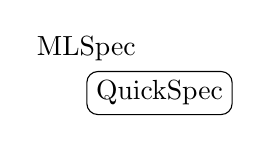
\begin{tikzpicture}[node distance = 2cm, auto]
        \node (mlspeclabel) {MLSpec};
        \node [block, anchor=north west, fill=white] at (mlspeclabel.south) (qs) {QuickSpec};
      \end{tikzpicture}
    };

    \node [block, below of=mlspec] (user) {User};

    \path [line] (hackage)    -- (cabal);
    \path [line] (cabal)      -- (sorting);
    \path [line] (sorting)    -- (clustering);
    \path [line] (clustering) -- (mlspec);
    \path [line] (mlspec)     -- (user);
  \end{tikzpicture}
  \caption{Components of the ML4HS theory exploration system. Custom components are shaded, arrows indicate data flow.}
  \label{fig:ml4hs}
\end{figure}

\subsection{\textsc{AST Plugin}}
\label{sec:astplugin}

The GHC compiler provides mechanisms for parsing Haskell source code and converting it to Core. It also includes a \emph{renaming} transformation, which resolves global identifiers into a canonical form. This allows us to spot repeated use of a term, across multiple modules and packages, with a simple syntactic equality check.

Since we are interested in comparing definitions based on the terms they reference, building our framework on top of GHC seems like a promising approach. Indeed, \hspec{} already invokes GHC's API to obtain the definitions of Haskell functions, in order to transform them into a form suitable for ATP systems. However, our initial experiments showed that this technique is too fragile for use on many real Haskell projects.

This is due to many projects having a complex module structure, requiring particular GHC flags to be given, or using pre-processors such as \texttt{cpp} and Template Haskell to generate parts of their code. All of this complexity means that invoking GHC ``manually'' via its API is unlikely to obtain the definitions we require.

Thankfully there is one implementation detail which most Haskell packages agree on: the Cabal build system. All of the above complexities will be specified in a package's ``Cabal file'', such that the \texttt{cabal configure} and \texttt{cabal build} commands are very likely to work for most packages, without any extra effort. This shifted our focus to augmenting GHC and Cabal, such that definitions can be collected during the normal Haskell build process.

GHC provides a plugin mechanism for manipulating Core during a build, intended for optimisation passes, which we use to inspect definitions as they are being compiled. We provide a plugin called \textsc{AstPlugin} which emits a serialised version of each Core definition to the console (to satisfy the type system, it also implements a dummy ``optimisation'' which returns the Core unchanged).

Compared to Haskell, Core is a much simpler language and its representation is relatively stable compared to many existing representations of Haskell (which often change to support various language extensions). Three areas which make Core difficult to handle are:

\begin{description}
  \item{Type variables}: Parametric polymorphism (described in more detail in \S \ref{sec:haskelldesc}) can be thought of as values being parameterised by type-level objects. In System F, this is represented explicitly by a special abstraction form $\Lambda$, distinct from the $\lambda$ used for values. Core only has one abstraction form, \CLam, for both types and values. This alters function properties like arity.

  \item{Unified namespace}: Haskell has distinct namespaces for values, types, data constructors, etc. Since Core does not make these distinctions, names may become ambiguous. For example, a type parameter \hs{t} may be confused with a function argument \hs{t}. To prevent this, overlapping namespaces are distinguished by prefices which are distinct from the available names; for example a type class constraint \hs{Ord t} may give rise to a binder $\CLam\ \hs{"\$dOrd"}$ in Core, which is guaranteed not to conflict since this name would be invalid in Haskell. This causes difficulties when looking up names, as these prefixed forms do not easily map back to the Haskell source.

  \item{Violating encapsulation}: Although Haskell allows names to be \emph{private} to a module, when compiling Core we have full access to private definitions, as well as references to private names from within other definitions. Hence the definitions we receive from \textsc{AstPlugin} will include private values which we cannot import into a theory exploration tool.
\end{description}

In practice, we work around these issues with a post-processing stage: for each named definition appearing in the output of \textsc{AstPlugin}, we attempt to reference that name within the GHCi interpreter. Names with the above problems will cause an error, and are discarded.

The result of building a Haskell package with \textsc{AstPlugin} enabled is a database of Haskell definitions, similar in some respects to \textsc{Hoogle} \cite{mitchell2008hoogle}. Definitions are indexed by a combination of their package name, module name and binding name. The definitions themselves are s-expressions representing the Core AST, with non-local references replaced by a combination of package name, module name and binding name, which makes it trivial to look up references in the database. Each definition also has an associated arity and type, obtained during the post-processing step mentioned above.

\subsection{Toplogical Sorting}

As described in \S \ref{sec:symbolstofeatures}, we must topologically sort the output of \textsc{AstPlugin} in order for our recurrent clustering to be well-founded. Since our database keys (containing the package, module and binding names, as described above) match our representation of non-local references, it is simple to walk each syntax tree to obtain the set of references it makes. In addition, the resulting set of (identifier, list-of-referenced-identifiers) pairs exactly matches the (vertex, list-of-successor-vertices) format used to represent directed graphs by the popular \hs{containers} library which ships with GHC. This provides an implementation of topological sort for strongly connected components, which we use as-is. A simple shell script loops through these SCCs, invoking the recurrent clustering component for each and appending the resulting features and clusters to the database.

\subsection{Feature Extraction}

The implementation of our feature extraction algorithm is a rather direct translation of the description given in \S \ref{sec:contributions} into Haskell. We parse the s-expressions generated by \textsc{AstPlugin} into algebraic data types which correspond directly to the definitions in Figure \ref{fig:coresyntax}; this is routine, so we omit the details for brevity. Similarly, we can represent rose trees with a datatype corresponding to the definition given in \S \ref{sec:expressionstovectors}:

\begin{haskell}
data RoseTree = Node Feature [RoseTree]
\end{haskell}

For simplicity we use the representation \hs{Feature = Int}, as we do not have fractional values. Since we represent the symbols $expr$, $id$, etc. from Figure \ref{fig:coresyntax} using different datatypes, we cannot write one big definition of $toTree$ or $\phi$ which works on all tokens. Each case shown in Figure \ref{fig:totree} and equations \ref{eq:feature}, \ref{eq:localfeature} and \ref{eq:globalfeature} appears in the implementation, although they are spread across several functions.

To support looking up local identifiers, our implementation of $toTree$ takes a context as argument, extending it as required. As an example of the complexity this adds, here is the \CCase\ branch of $toTree$:

\begin{lstlisting}[language=Haskell, xleftmargin=0pt, xrightmargin=0pt]
toTree :: Context -> Expr -> RoseTree
toTree ctx x = case x of
  ...
  Case e l as -> Node fCase (toTree ctx e : map (toTreeAlt (l:ctx)) as)
  ...
\end{lstlisting}

Breaking this down we can see \hs{fCase} representing the value of $\feature{\CCase}$, and a list of sub-trees defined in parentheses. The first subtree is a straightforward recursive call in an unmodified context: \mbox{\hs{toTree ctx e}}. The rest of the list is formed by applying the function \mbox{\hs{toTreeAlt (l:ctx)}} to each element of the list \hs{as} of \CAlt\ clauses.

The \hs{toTreeAlt} function contains those cases of $toTree$ which handle symbols in $alt$. We prepend the identifier \hs{l} to the context, to get the extended context \hs{l:ctx}. This is because \hs{l} will be bound the value of \hs{e}, in order to avoid re-computing its value several times.

The other clauses are handled in a similar way. The trickiest is the \CLet\ clause, since the local identifiers aren't directly available; we must extract them from their \CRec, \CNonRec\ and \CBind\ wrappers first, which we do using helper functions.

As shown above, the values from equations \ref{eq:feature} are encoded directly in $toTree$. For $phi(l \in \mathcal{L})$ we use standard Haskell functions to look up the required indices in the context:

\begin{lstlisting}[language=Haskell, xleftmargin=0.1\textwidth, xrightmargin=0.1\textwidth]
phiL :: Context -> Local -> Feature
phiL ctx x = case elemIndex x ctx of
  Nothing -> error (concat ["Local '", show x,
                            "' not in context '",
                            show ctx, "'"])
  Just i  -> (2 * alpha) + i
\end{lstlisting}

As explained in \S \ref{sec:symbolstofeatures}, local identifiers should always exist in the context. If this precondition doesn't hold, we abort the program with an error rather than continuing.

Global identifiers are kept as-is until we have access to the clusters from the last iteration. This takes place outside Haskell, using the \hs{jq} data processing tool.

Our implementation of $level$ exactly matches equation \ref{eq:level}:

\begin{haskell}
level :: Int -> RoseTree -> [[Feature]]
level 1 (Node f _)  = [f]
level n (Node _ ts) = concatMap (level (n-1)) ts
\end{haskell}

To produce feature vectors, we do not directly construct the matrix; instead we generate the rows and concatenate them together in one step, using the \hs{concatMap} function:

\begin{lstlisting}[language=Haskell, xleftmargin=0.1\textwidth, xrightmargin=0.1\textwidth]
featureVec :: Expr -> [Feature]
featureVec e = concatMap (\m -> pad (level m tree)) [1..r]
  where tree   = toTree [] e
        pad xs = take c (xs ++ repeat 0)
\end{lstlisting}

By providing \hs{featureVec} with the latest set of clusters, read from the \textsc{AstPlugin} database, we turn Core expressions into feature vectors, which are appended to the database.

We use the Weka system to perform our k-means clustering, as it is widely used, including by ML4PG. We select all feature vectors from our database, and write them in CSV format for Weka to process. The Weka CLI command is invoked, which appends a cluster number to each of these feature vectors; we read these off and append them to the database. As long as more SCCs remain unprocessed, we keep looping this process, using the database to communicate between the feature extraction and clustering phases.

\subsection{\textsc{MLSpec}}
\label{sec:mlspec}

We cannot supply these clusters as-is to \qspec{}, since it must be provided with a \emph{signature}. These are constructed by our \textsc{MLSpec} tool, using information from the \textsc{AstPlugin} database. Tasks performed by \textsc{MLSpec} include:

\begin{itemize}
  \item{Monomorphising}: Given values of polymorphic type, e.g. \hs{safeHead :: forall t. [t] -> Maybe t} and \hs{[] :: forall t. [t]}, a testing-based system like \qspec{} is unable to evaluate these expressions without instantiating the variable \hs{t} to a specific type. Such an instantiation is called \emph{monomorphising}, and in the case of \textsc{MLSpec} we build on previous work in \qcheck{} by attempting to instantiate all type variables to \hs{Integer}. We discard those cases where this is invalid, such as variable \emph{type constructors} (e.g. \hs{forall c. c Bool -> c Bool}) or incompatible class constraints (e.g. \hs{forall t. IsString t => t}).

  \item{Qualification}: All names are \emph{qualified} (prefixed by their module's name), to avoid most ambiguity. There is still the possibility that multiple packages will declare modules of the same name, although this is rare as it causes problems for any Haskell programmer trying to use those modules. In such cases the exploration process simply aborts.

  \item{Variable definition}: Once a \qspec{} theory has been defined containing all of the given terms, we inspect the types it references and append three variables for each to the theory (enough to discover laws such as associativity, but not too many to overflow the limit of \qspec{}'s exhaustive search).

  \item{Sandboxing}: One difficulty with Haskell's packaging infrastructure is that all required packages and modules must be provided up-front, usually by specification in a Cabal file. Since \textsc{MLSpec} builds signatures \emph{dynamically}, depending on the cluster information it is given, we do not know what packages it may need. To work around this problem, \textsc{MLSpec} invokes \qspec{} for each cluster using a library we have built called \texttt{nix-eval}. This provides an \texttt{eval} function, like those commonly found in dynamic languages such as Python and Javascript, for evaluating Haskell expressions. The key feature of \texttt{nix-eval} is that these Haskell expressions may reference packages that are not installed on the system. When such expressions are evaluated, these packages will be automatically downloaded and installed into a sandbox using the Nix package manager, and GHC will be invoked in this sandbox to perform the evaluation.

\end{itemize}
